\documentclass[11pt, oneside]{article} 
\usepackage{geometry}
\geometry{letterpaper} 
\usepackage{graphicx}
	
\usepackage{amssymb}
\usepackage{amsmath}
\usepackage{parskip}
\usepackage{color}
\usepackage{hyperref}

\graphicspath{{/Users/telliott_admin/Tex/png/}}
% \begin{center} 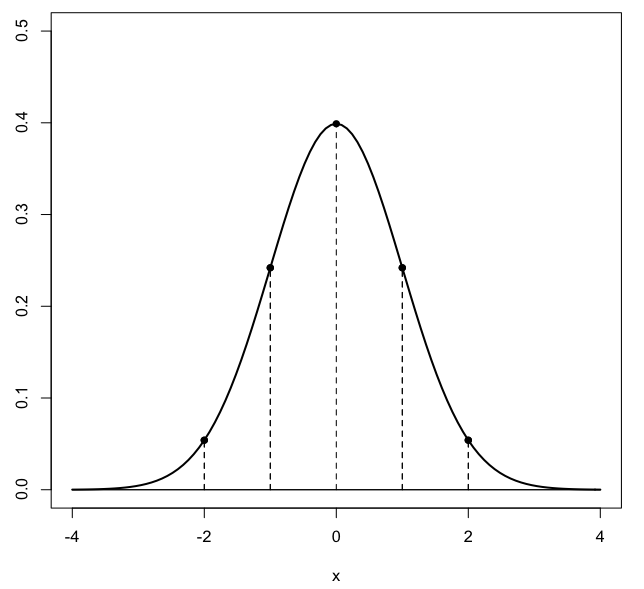
\includegraphics [scale=0.4] {gauss3.png} \end{center}

\title{Limits and continuity}
\date{}

\begin{document}
\maketitle
\Large

\section{Limits}

Consider the graph of a function $f(x)$.  We might choose a power of $x$ similar to $y = x^2$ or $y = x^3 - x$, which affirmatively has two properties that are of interest here:  continuity and differentiability.
\begin{center} 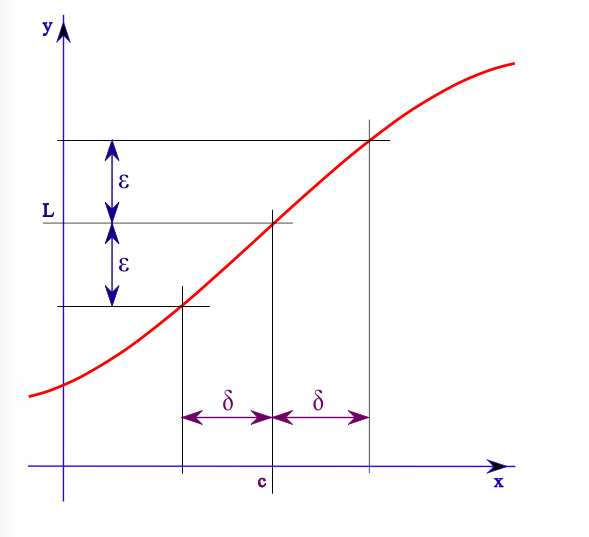
\includegraphics [scale=0.35] {epsilon-delta.png} \end{center}
We focus on the neighborhood of a point on the $x$-axis, $x=c$.

By inspection of the graph we see that the value of $f(x)$ at $c$ is equal to $L$, and furthermore, for points near $c$, the value of $f$ at those points is not too different from $L$.

We would like to say that the \emph{limit} of $f(x)$ as $x$ \emph{approaches} $c$ is equal to $L$.  The idea is that we can make $f(x)$ as close to $L$ as we please, provided we choose $x$ sufficiently close to $c$.

\begin{quote}When the values successively attributed to a variable approach indefinitely to a fixed value, in a manner so as to end by differing from it by as little as one wishes, this last is called the limit of all the others.  ---Cauchy\end{quote}

\begin{center} 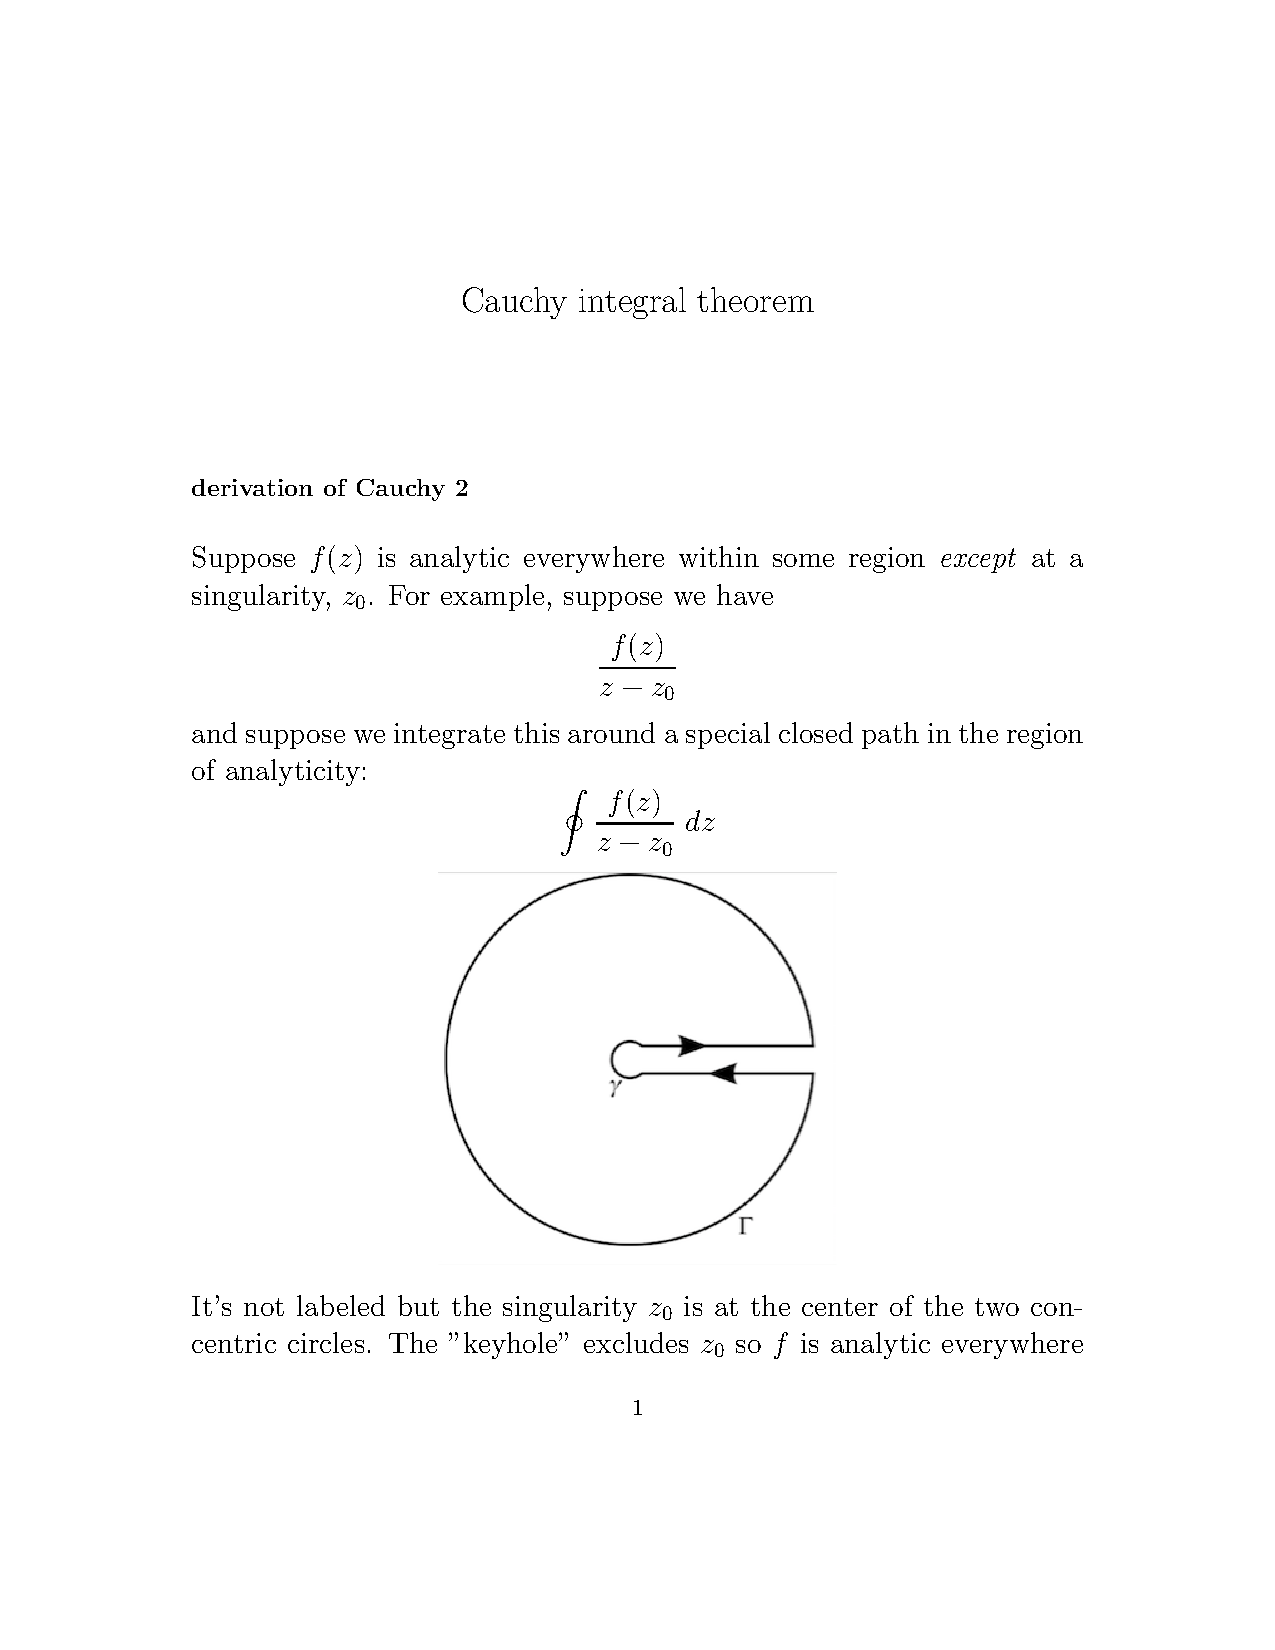
\includegraphics [scale=0.3] {Cauchy} \end{center}

Modern mathematicians don't like that word "approach", which conjures up movement and the involvement of time, and they don't like reasoning from what they see in a graph, in part because no graph can show the whole function for the general case.  Instead we will use an algebraic method from the formal apparatus of calculus.

There are two equivalent approaches, neighborhoods, and epsilon-delta formalism.  Let's look at neighborhoods briefly first.
\subsection*{neighborhoods}

First, an \emph{interval} between two real numbers $a$ and $b$ ($a < b$) contains every real number $a < x < b$.
\[ (a,b) = x \ | \ a < x < b \]
The "$|$" means $x$ "such that" the condition $a < x < b$ holds.

A \emph{closed} interval $[a,b]$ includes the endpoints ($a \le x \le b$), while an \emph{open} interval $(a,b)$ excludes them.  Half-open intervals like $[a,b)$ may be defined, and an interval with $\pm \ \infty$ as an endpoint is always open on that end, for example:  $[a,\infty)$.

Any open interval with a point $p$ as its midpoint is called a \emph{neighborhood} of $p$.  The distance $r$ from $p$ to the boundary of a particular neighborhood may be large or very very small.  We denote a neighborhood of $p$ as $N(p)$.
\[ N(p) = x \ \text{ such that } \ |x-p| < r \].

To say that the limit $f(x) \rightarrow L$ exists, we mean that for every neighborhood $N_1(L)$, there exists some neighborhood $N_2(p)$ such that $f(x) \in N_1(L)$ whenever $x \in N_2(p)$.  

For a limit, we exclude the point $x = p$.  It is not necessary that $f(p) = L$.

The idea of a neighborhood is a nice abstraction to hide the apparatus of modern calculus, which we look at next.
\begin{center} 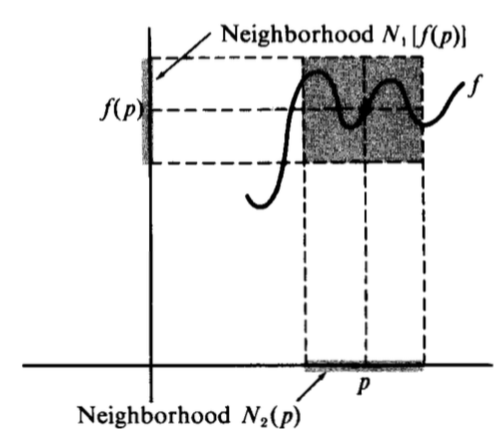
\includegraphics [scale=0.4] {neighborhood.png} \end{center}

\subsection*{epsilon-delta game}
The formal method uses numbers called $\epsilon$ and $\delta$ and is originally due to Bolzano.

We say that, \emph{if} for all points $x$ within a specified distance $\delta$ of $c$, we find that $f(x)$ lies within a specified distance $\epsilon$ from $L$, \emph{then} the limit is $L$.

To do this we must choose $\epsilon$ first.  That's why I call it a game.  Why don't you go first?  Choose $\epsilon$, which provides a constraint on how close to $L$ you want the value of $f(x)$ to be:  you require that  $|f(x) - L| < \epsilon$.  The \emph{distance} from $f(x)$ to $L$ must be less than $\epsilon$.

Now that I know your $\epsilon$, I must try to find a suitable $\delta$.  If I can, then you get another chance, and will presumably choose a smaller $\epsilon$.  

If I can show that it is possible to find a $\delta$ to guarantee that your constraint is satisfied for \emph{all} values of $\epsilon > 0$ \emph{no matter how small}, then I win and the limit exists.  If not, it doesn't.

Here is the formal definition:
\[ \forall \ \epsilon > 0, \exists \ \delta > 0 \ | \ \forall \ x \]
For all (arbitrary) $\epsilon$, there exists $\delta > 0$ such that for all $x$ satisfying
\[ \ 0 < | x - c| < \delta \Rightarrow | f(x) - L | < \epsilon \]

We describe the limit defined above by saying that
\[ \lim_{x \rightarrow c} f(x) = L \]
The limit as $x$ tends to, or approaches, $c$ is equal to $L$.

Important points about limits:

$\bullet$  We do not require that $f(c) = L$.

The function $f(x)$ may or \emph{may not} have the value $L$ at $x=c$ and the limit can still exist and be equal to $L$.  Suppose we have $f(x) = x$, whose graph is the line $y=x$, except that we decide to define $f(0) = 1$, leaving a hole in our line $y=x$ at the point where $x=0$.  The limit of $f(x)$ at $x=0$ is equal to $0$, despite the fact that $f(0) = 1$.

Alternatively, suppose that we only allow values of $x$ in the open interval $(a,b)$, and the limit $x \rightarrow a +$ (from the right) does exist.  Since we have restricted the domain of $f$ to values $x > a$ the limit $x \rightarrow a -$ certainly does not exist, and in fact the left-hand endpoint $a$ is not in the domain of $f$.

We say that such a limit ($x \rightarrow a +$) is a \emph{one-sided} limit.  If the two one-sided limits do not agree at a particular value of $c$, then the (two-sided) limit does not exist.

$\bullet$  Limits must be unique.

\subsection*{proof}
If
\[ \lim_{x \rightarrow c} f(x) = L \]
\[ \lim_{x \rightarrow c} f(x) = M \]
Then $M = L$.

The proof is by contradiction.  Suppose $L \ne M$.  Let
\[ \epsilon = \frac{|L - M|}{10} \]

There is an $N_1$ such that if $n > N_1$, then $|a_n - L| < \epsilon$.

There is an $N_2$ such that if $n > N_2$, then $|a_n - M| < \epsilon$.

Let $N = $ max($N_1,N_2)$.  

If $n > N$ then $|a_n - L| < \epsilon$ and $|a_n - M| < \epsilon$.

By the triangle inequality:
\[ |L - M| \le |a_n - L| + |M - a_n| \]
But also
\[ |a_n - L| + |M - a_n| < \frac{2}{10} |L - M| \]
so
\[ |L - M| \le \frac{2}{10} |L - M| \]
which is impossible.

We have reached a contradiction.  Therefore, $L = M$.

$\square$

$\bullet$  We allow the existence of a limit as $x$ approaches $\infty$
\[ \lim_{x \rightarrow \infty} f(x) = L \]
To define this limit, play the epsilon-delta game (typically, using $c$ instead of $\delta$) and say that if, when $x > c$, $|f(x) - L| < \epsilon$, the limit "at" $\infty$, or as $x$ \emph{tends to} $\infty$, exists and has the value $L$.

\subsection*{example:  floor}
Consider the "floor" function, which is defined on the real numbers and has the value of the largest integer less than or equal to $x$.
\begin{center} 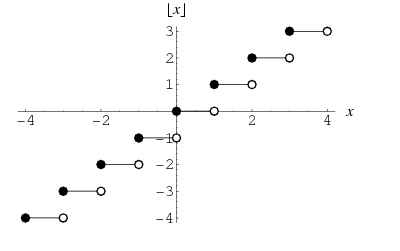
\includegraphics [scale=0.75] {floor.png} \end{center}
The floor function has one-sided limits (from the right) at integral values of $x$, but the limit at $x=2$, for example, does not exist, because those two one-sided limits are not the same.

\subsection*{example:  inverse}
Consider the function $f(x) = 1/x$.  This function is undefined at $x=0$ since division by zero is not defined.  As $x$ gets close to zero from the right, $1/x$ takes on larger and larger positive values.

Some people will say that limits can have infinite values.  In the case of $f(x) = 1/x$, informally, we accept that the limit as $x \rightarrow 0+$ exists and has the value $\infty$.  Speaking more formally, we might say that the function "diverges" or "grows without bound".

In any case since for $f(x) = 1/x$
\[ \lim_{x \rightarrow 0+} \ne \lim_{x \rightarrow 0-} \]
so the limit as $x \rightarrow 0$ does not exist (abbreviated D.N.E.).

\subsection*{example:  sine of 1/x}
The trigonometric functions sine and cosine are, of course, periodic.  For any value of $\theta$
\[ \sin \theta = \sin ( \theta \pm 2 \pi) \]
The maximum values of the sine function (for $\theta > 0$) occur at
\[ \theta = \frac{\pi}{2},  \frac{5\pi}{2}, \frac{9\pi}{2}, \frac{13\pi}{2} \dots \]
The corresponding maximum values of $\theta = 1/x$ occur at
\[ x = \frac{2}{\pi}, \frac{2}{5 \pi}, \frac{2}{9 \pi}, \frac{2}{13 \pi} \dots \]
The corresponding decimal values are approximately
\[ x = 0.6366, 0.1273, 0.0707, 0.0490 \]
As $\pi/2 + 2k\pi$ gets larger, the corresponding values for the inverse get smaller, and more closely spaced together.

Now, $1/x$ grows without bound as $x \rightarrow 0$.  This means that there is an infinite number of places where the value of the function $\sin(1/x)$ is equal to $1$ and indeed, takes on all possible values in its range $[-1,1]$, and this occurs more and more rapidly as $x \rightarrow 0$.

In short, the value oscillates and does so more extremely the closer $x \rightarrow 0$.
\begin{center} 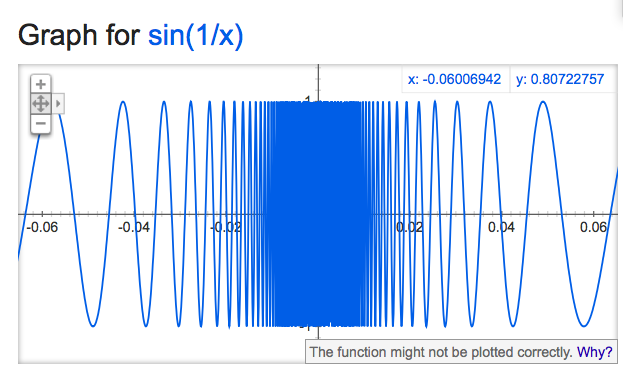
\includegraphics [scale=0.4] {sinxinverse.png} \end{center}
The limit as $x \Rightarrow 0$ D.N.E.

\section{Calculating limits}

The limit of a function $f(x)$ at a point $a$ is written
\[ \lim_{x \rightarrow a} f(x) = L \]

The formal definition is:
\[  \forall \ \epsilon > 0, \exists \ \delta > 0 \ | \ \forall \ x, \]
\[ 0 < | x - a| < \delta \Rightarrow | f(x) - L | < \epsilon \]

You tell me the $\epsilon$ you require with $| f(x) - L | < \epsilon$, and I will try to find the right $\delta$.

For a typical function, it's a good guess that $L = f(a)$.
\[ | f(x) - f(a) | < \epsilon \]
which we can write without the absolute value bars (see Triangle write-up):
\[ -\epsilon <  f(x) - f(a) < \epsilon \]

\subsection*{example 1}
Suppose $f(x) = 3x$ and we're interested in the point $a = 5$.  Then set $L = f(a) = 15$.
\[ -\epsilon <  f(x) - f(a) < \epsilon \]
\[ -\epsilon <  3x - 15 < \epsilon \]
\[ - \frac{\epsilon}{3} <  x - 5 < \frac{\epsilon}{3} \]
If we set $\delta = \epsilon/3$ we'll be good.  And in general for a function $f(x) = cx$ with $c$ a constant, at the point $a$, we can use
\[ | x | - a <  \frac{\epsilon}{c} \]

\subsection*{example 2}
Suppose $f(x) = x^2$ and we're interested in the point $a = 2$.  Then set $L = f(a) = a^2 = 4$.
\[ -\epsilon <  f(x) - f(a) < \epsilon \]
\[ -\epsilon <  x^2 - a^2 < \epsilon \]
or
\[ | x^2 - a^2 | < \epsilon \]

Now we argue as follows:
\[ | x^2 - a^2|  = | (x - a)(x + a) | \]
\[ = |x-a| \ |x + a| \]
(The last step follows from $|xy| = |x||y|$ which is true even if $xy < 0$).

To get started suppose we require that \emph{at least}
\[ | x - a | < 1 \]
\[ -1 < x - a < 1 \]
\[ a - 1 < x < a + 1 \]
\[ 2a - 1 < x + a < 2a + 1 \]
\[ |x + a| < 2a + 1 \]
Then going back to 
\[ |x-a| \ |x + a| < \epsilon \]
\[ |x-a| \ |x + a| < |x - a| \ (2a + 1) < \epsilon \]
and
\[ |x - a| < \frac{\epsilon}{(2a + 1)} \]
Remembering the first condition we set:
\[ |x - a| < \min ( \frac{\epsilon}{(2a + 1)}, 1) = \delta \]
And what we notice is that for $f(x) = x^2$, at least for some $a$ (and depending on the value of $\epsilon$ that is chosen), the value of $\delta$ required depends on $a$.

That should not be too surprising.
\begin{center} 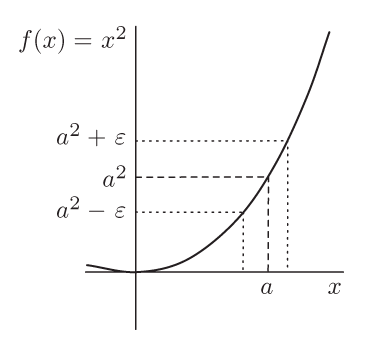
\includegraphics [scale=0.6] {limits2.png} \end{center}
The same $\epsilon$ will require a smaller $\delta$ the farther out we go on the curve.

\subsection*{example 3}
Now consider the inverse function $f(x) = 1/x$.  Suppose we're interested in the point $a = 3$ where we expect the limit to be $L = 1/3$.  For this to be true we must guarantee that
\[ | \frac{1}{x} - \frac{1}{3} | < \epsilon \]
for arbitrary $\epsilon$.

Factor
\[ | \frac{1}{x} - \frac{1}{3} | = | \frac{3 - x}{3x} | = \frac{1}{3} \ \frac{1}{|x|} \ |3 - x|   \]

We showed in the write-up on the triangle inequality that $|a - x| = |x - a|$ so
\[ =  \frac{1}{3} \ \frac{1}{|x|} \ |x - 3|   \]

Here, we need to make sure that $|x|$ is not too \emph{small}, so $1/|x|$ is not too large.

First require that $|x - 3| < 1$ .  Then
\[ -1 < x - 3 < 1 \]
\[ 2 < x < 4 \]
\[ \frac{1}{4} < \frac{1}{x} < \frac{1}{2} \]
This means that $1/x > 0$ so
\[ \frac{1}{|x|} = \frac{1}{x} < \frac{1}{2} \]

We now have
\[ | \frac{1}{x} - \frac{1}{3} | = \frac{1}{3} \ \frac{1}{|x|} \ |3 - x|   \]
provided $|x - 3| < 1$ and also with this condition $1/|x| < 1/2$ so
\[  | \frac{1}{x} - \frac{1}{3} | < \frac{1}{6} \ |x - 3| \]
Hence if $\delta = |x - 3| < 6 \epsilon$, the above expression is $< \epsilon$ and we're done.  Officially we need:
\[ |x - 3| < \min \ (6 \epsilon, 1) \]

\section{Combining Limits}

Assume that
\[ \lim_{x \rightarrow c} f(x) = L \]
\[ \lim_{x \rightarrow c} g(x) = M \]

We want to show that
\[ \lim_{x \rightarrow c} f(x) + g(x) = L + M \]
The limit of the sum is the sum of the limits.

Let $\epsilon > 0$ be arbitrary.

Then the existence of the limits means that
\[ \forall \ \epsilon, \exists \ \delta_1 > 0 \ | \ \forall \ x, \ 0 < | x - c| < \delta_1 \rightarrow | f(x) - L | < \epsilon/2 \]
and
\[ \forall \ \epsilon, \exists \ \delta_2 > 0 \ | \ \forall \ x, \ 0 < | x - c| < \delta_2 \rightarrow | g(x) - M | < \epsilon/2 \]
Let
\[ \delta = \text{ min } (\delta_1, \delta_2) \]
Now for $|x - c| < \delta$:
\[ | f(x) - L + g(x) - M| < \epsilon \]
But by the triangle inequality the left-hand side is 
\[ | f(x) - L| + |g(x) - M|  \le | f(x) - L + g(x) - M|  \]
so
\[   | f(x) - L| + |g(x) - M| < \epsilon \]
which proves the theorem.

\subsection*{proof of the product rule for limits}
Assume that
\[ \lim_{x \rightarrow c} f(x) = L \]
\[ \lim_{x \rightarrow c} g(x) = M \]

We want to show that
\[ \lim_{x \rightarrow c} f(x) \cdot g(x) = LM \]
The limit of the product is the product of the limits.

We need to show that
\[ f(x) \cdot g(x) - LM \]
is small.  

Subtract $L g(x)$ and add it back
\[ f(x) \cdot g(x) - LM = f(x) \cdot g(x) - L g(x) + L g(x) - LM \]
\[ = (f(x) - L) g(x) + L (g(x) - M ) \]
Take the absolute value on both sides
\[  |f(x) \cdot g(x) - LM| = |(f(x) - L) \cdot g(x) + L \cdot (g(x) - M )| \]
Use the triangle inequality to split up the sum:
\[ \le |(f(x) - L) \cdot g(x)| + |L \cdot (g(x) - M )| \]
This can be further massaged to 
\[  =| f(x) - L | \cdot |g(x)| + |L| \cdot |g(x) - M | \]
Write the whole thing:
\[ |f(x) \cdot g(x) - LM| \le |(f(x) - L) | | g(x) | + | L | | (g(x) - M )| \]

Now, play the epsilon-delta game:  you pick $\epsilon$ and then I concentrate on a region so close to $c$ that
\[ |f(x) - L | < \epsilon \]
and
\[ |g(x) - M | < \epsilon \]

If your epsilon is too large it would mess things up (why?), so in that case I will pick $|g(x) - M| = 1$.

Then I have
\[ |f(x) - L | < \epsilon \]
\[ |g(x) - M | < \epsilon \]
\[ |g(x)| < |M| + 1 \]

Go back to the equation we obtained above
\[ |f(x) \cdot g(x) - LM| \le |(f(x) - L) | | g(x)| + | L | | (g(x) - M )| \]
substitute on the right-hand side
\[ |(f(x) - L) | | g(x)| + | L | | (g(x) - M )| \]
\[ \le \epsilon \ (|M| + 1) + | L | \ \epsilon \]
\[ \le \epsilon \ (|M| + |L| + 1) \]
That is:
\[ |f(x) \cdot g(x) - LM| \le \epsilon \ (|M| + |L| + 1) \]

as Adrian Banner says in \emph{Calculus Lifesaver}:

\begin{quote}
That's almost what I want!  I was supposed to get $\epsilon$ on the right-hand side, but I got an extra factor of $|M| + |L| + 1$.  This is no problem---you just have to allow me to make my move again, but this time I'll make sure that $|f(x) - L|$ is no more than $\epsilon/2(|M| + |L| + 1)$, and similarly for $|g(x) - M|$.  Then when I replay all the steps, $\epsilon$ will be replaced by $\epsilon/(|M| + |L| + 1)$, and at the very last step, the factor $|M| + |L| + 1$ will cancel out and we'll just get our $\epsilon$.  So we have proved the result.
\end{quote}

\subsection*{More formal proof of the product rule}

Suppose that 
\[ \lim_{x \rightarrow c} f(x) = L \]
\[ \lim_{x \rightarrow c} g(x) = M \]

To prove:
\[ \lim_{x \rightarrow c} f(x) \cdot g(x) = LM \]

\subsection*{Proof}
Let $\epsilon > 0$.  By the definition of limits we can find three numbers $\delta_1$, $\delta_2$ and $\delta_3$ such that

if $0 < |x - c| < \delta_1$:
\[ |f(x) - L| < \frac{\epsilon}{2(1 + |M|)} \]
if $0 < |x - c| < \delta_2$:
\[ |g(x) - M| < \frac{\epsilon}{2(1 + |L|)} \]
and third, if $0 < |x - c| < \delta_3$:
\[ |g(x) - M| < 1 \]

Now write
\[ |g(x)| = |g(x) - M + M| \]
use the triangle inequality
\[ |g(x)| \le |g(x) - M| + |M|\]
Then according to (3), if if $0 < |x - c| < \delta_3$:
\[ |g(x) \le 1 + |M|  \]

Choose $\delta = \min \{\delta_1,\delta_2,\delta_3\}$.

Then if $0 < |x - c| < \delta$:
\[ |f(x) \cdot g(x) - LM| = |f(x) \cdot g(x) - L \cdot g(x) + L \cdot g(x) - LM| \]
by the triangle inequality (again)
\[ \le |f(x) \cdot g(x) - L \cdot g(x)| + |L \cdot g(x) - LM| \]
The next step is to factor (see below):
\[ \le |g(x)| |f(x) - L| + |L| |g(x) - M| \]
\[ < (1 + |M|) \ \frac{\epsilon}{2(1 + |M|)} + (1 + |L|) \ \frac{\epsilon}{2(1 + |L|)} \]
\[ < \frac{\epsilon}{2} + \frac{\epsilon}{2} \]
\[ |f(x) \cdot g(x) - LM| < \epsilon \]
which completes the proof.

\section{Continuity}

Continuity has an intuitive definition:  if we can graph a function \emph{without lifting our pencil from the paper}, then the function is continuous.

Here are some graphs showing examples of how continuity can fail.
\begin{center} 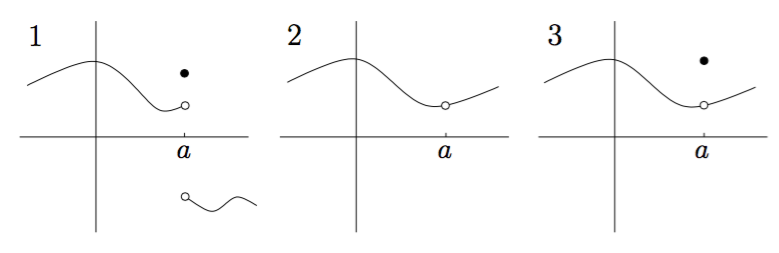
\includegraphics [scale=0.5] {continuity_failure.png} \end{center}
\begin{center} 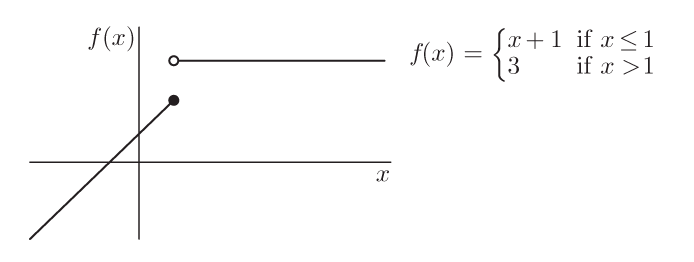
\includegraphics [scale=0.5] {continuity_failure2.png} \end{center}

For a function to be continuous at a point $x=c$, we imagine that if we vary $x$ in neighborhood of $c$, then $f(x)$ should not change in value by too much.

Again, we will call that value $L$, the limit of $f(x)$ as $x \rightarrow c$.  For $L$ to exist we require that the two one-sided limits be equal.  

In addition, it must also be true that $f(c) = L$.

\subsection*{fancy definitions}
If we had not previously developed the concept of a limit, we might proceed as follows:  a function $f : \mathbb{R} \rightarrow \mathbb{R}$ is continuous at $c \in \mathbb{R}$ if and only if 
\[ \forall \ \epsilon > 0 \ \exists \ \delta > 0 \ \text{ such that, if } |x-c| < \delta, \text{ then } |f(x) - f(c)| < \epsilon \]

Above we talked about functions, here is a definition that involves sequences.

Let $f:  \mathbb{R} \rightarrow \mathbb{R}$ be a function and $L \in \mathbb{R}$.  We say that $f$ is continuous at $L$, if, whenever $(a_n)$ is a sequence that converges to $L$, then the sequence $(b_n)$ defined by $f(a_n)$ also converges and its limit is equal to $f(L)$.  We say that $f$ is continuous if it is continuous at all $L \in \mathbb{R}$.

\subsection*{example:  absolute value}
An algebraic definition of the absolute value function is piecewise:
\[ |x| =
\begin{cases}
\ \ x, \ \ \ x \ge 0  \\
-x, \ \ \ x < 0
\end{cases}
\]
\begin{center} 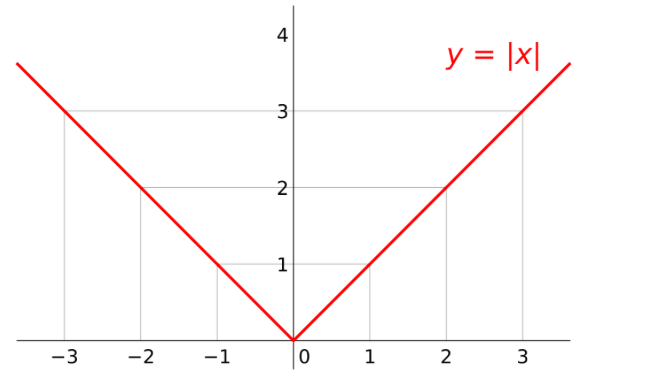
\includegraphics [scale=0.4] {abs.png} \end{center}
The function $f(x) = |x|$ is continuous at $x=0$ because the two one-sided limits exist and are equal to each other.  They are also equal to $f(0) = 0$.

\subsection*{example:  constant}
Suppose $f(x) = a$ for some real number $a$.  Then no matter what $\epsilon$ is chosen and no matter what real number $c$ is chosen
\[ f(x) = f(c) = a \]
so
\[ |f(x) - f(c)| < \epsilon \]

\subsection*{example:  x}
Suppose $f(x) = x$.  
\[ \lim_{x \rightarrow c} f(x) = c  = f(c) \]
so $f$ is continuous at $c$.

Or choose $\delta = \epsilon$.  Then, if $|x-c| < \delta$
\[ c- \delta < x < c + \delta \]
\[ f(x) = x \]
\[ f(x) - c < \delta = \epsilon \]
\[ | f(x) - c | < \epsilon \]
so $f$ is continuous at $c$

\subsection*{example:  constant factor}
Suppose $f(x) = cx$ ($c \in \mathbb{R}$).  Use the $\epsilon-\delta$ game to prove that $f$ is continuous.

Proof:  the function "stretches" $x$ by a factor of $c$.  Hence $\delta$ will also be stretched.  Set $\delta = \epsilon/c$.  Then, if $|x-a| < \delta$ we have
\[ |f(x) - f(a)| = |cx - ca| = c |x-a| < c \delta = c \epsilon / c = \epsilon \]
Hence $f$ is continuous at every $a \in \mathbb{R}$.

\subsection*{example:  product rule}
How to prove that $f(x) = x^2$ is continuous?  One way is to try adjusting $\delta$ based on the value of $a$ (e.g. min $(| \sqrt{a^2 + \epsilon} \ \pm a|)$), but a better way is to invoke the product rule.

If $f: \mathbb{R} \rightarrow \mathbb{R}$ and $g: \mathbb{R} \rightarrow \mathbb{R}$ are both continuous at $a \in  \mathbb{R}$, then $fg$ is continuous at $a$.

First, prove $f(x) = x$ is continuous.  Then define $f(x) = g(x) = x$.  So $x^2 = f(x) g(x)$ in continuous.

By induction then, all powers $f(x) = x^n$ are continuous.

\subsection*{proof of the product rule for continuity}
Let $f$ and $g$ be functions defined on an open subset of $\mathbb{R}$.  We have that $f$ and $g$ are both continuous at $c$ which means that
\[ \lim_{x \rightarrow c} f(x) = L \]
\[ \lim_{x \rightarrow c} g(x) = M \]
Then
\[ \lim_{x \rightarrow c} f(x) \cdot g(x) = \lim_{x \rightarrow c} f(x) \cdot \lim_{x \rightarrow c} g(x) = LM \]

To obtain this result we have used the product rule for limits. 

\subsection*{example:  inverse}
Consider the function $f(x) = 1/x$.  Above we pointed out that this function is undefined at $x=0$ since division by zero is not defined.  But there is nothing to stop us from defining the function piecewise, like so:

\[ f(x) = 
\begin{cases}
\frac{1}{x} \ \ x \ne 0 \\
0 \ \ x = 0 
\end{cases} \]

As $x$ gets close to zero from the right, $1/x$ continues to take on larger and larger positive values, but then dives to $0$ at $x=0$ and then further dives toward $-\infty$ as we pass to the left of zero.

Trick question:  give an example of a function $f : \mathbb{R} \rightarrow \mathbb{R}$ that is not continuous at zero.  If you said the inverse, that is not correct.  The reason is that the inverse is not $f : \mathbb{R} \rightarrow \mathbb{R}$ because \emph{it is not defined at zero}.

On the other hand, $f(x) = \sin(x)$ \emph{is} $f : \mathbb{R} \rightarrow \mathbb{R}$ even though the values actually output by the function are $f(x) \in [-1,1]$.  That interval is the \emph{image} of the function, any codomain so that the image is contained in the codomain will do.

\subsection*{example}
A famous (but weird) function is defined as
\[ f(x) =
\begin{cases}
1 \ \ \text{ if } x \in \mathbb{Q} \\
0 \ \ \text{ if } x \notin \mathbb{Q} 
\end{cases}
\]

As we said before, you can imagine that the graph of this function looks like a linear hairbrush, with spikes at each rational number.

However, any interval such as $[0,1]$, or $[0.001, 0.002]$ contains an infinite number of rational numbers, but an even larger infinite number of real numbers.  In other words, we only get the hairbrush image if we exclude denominators greater than some value.  And we get the exact same image if we blow up any portion of the graph.

This is hard to think about.

The first function is not continuous anywhere, but the following variant is:
\[ f(x) =
\begin{cases}
x \ \ \text{ if } x \in \mathbb{Q} \\
0 \ \ \text{ if } x \notin \mathbb{Q} 
\end{cases}
\]

Why?

\subsection*{uniform continuity}
The notion of continuity described so far is called "pointwise."  We first pick a point $c$, and then working near that point, we pick an $\epsilon$ and then a $\delta$ and so on.  A particular $\delta$ may be satisfactory for some values of $c$ and not for others.

One can pick a "one-size-fits-all" $\delta$ for some functions and intervals, but not always.  

Weierstrass and his student Heine developed the idea of "uniform continuity".

\begin{center} 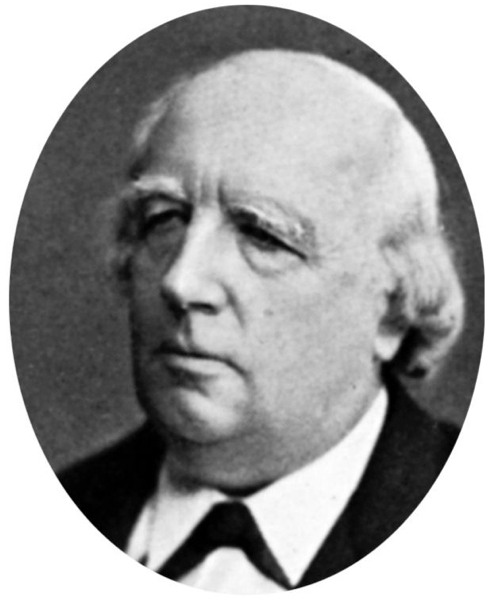
\includegraphics [scale=0.4] {Weierstrass} \end{center}
Weierstrass

A function $f$ is uniformly continuous on some domain if, for every $\epsilon > 0$, there exists a $\delta > 0$ so that, if $x$ and $y$ are any two points in the domain within $\delta$ units of one another, then $|f(x) - f(y)| < \epsilon$.  This $\delta$ must work everywhere in the domain.

It turns out that a function can be point-wise but not uniformly continuous.  Consider $f(x) = 1/x$ on the open interval $(0,1)$.  The problem is that the values of the function rise to $\infty$ as $x \rightarrow 0$.  Suppose you have some $\delta$ that works for a particular $\epsilon$ near point $c$.  We can always move far enough to the left to a new pair $x,y$ so that the rise in $f(x)$ for a change in $x$ of $\delta$ is $> \epsilon$.

However, Heine proved that a function continous on a closed, bounded interval $[a,b]$ must be uniformly continuous.  According to the internet, 
"a function is uniformly continuous on $(0,1)$ if and only if it can be extended continuously to $[0,1]$."


\end{document}  